\documentclass[11pt]{article}

%%%%%%%%%%%%%%Include Packages%%%%%%%%%%%%%%%%%%%%%%%%%%
\usepackage{xcolor}
\usepackage{mathtools}
\usepackage[a4paper, total={6in, 8in}, margin=1.25in]{geometry}
\usepackage{amsmath}
\usepackage{amssymb}
\usepackage{paralist}
\usepackage{rsfso}
\usepackage{amsthm}
\usepackage{wasysym}
\usepackage[inline]{enumitem}   
\usepackage{hyperref}
\usepackage{tocloft}
\usepackage{titlesec}
\usepackage{colortbl}
\usepackage{wrapfig}
\usepackage{pdfpages}
%%%%%%%%%%%%%%%%%%%%%%%%%%%%%%%%%%%%%%%%%%%%%%%%%%%%%%%%



\begin{document}
\Large \noindent \textbf{Physics 5A Discussion (Week 1)}\\
\normalsize
Department of Physics and Astronomy, UCLA\\
\noindent\rule{8cm}{0.4pt}\\

%\begin{wrapfigure}[8]{r}{0.4\textwidth}
%  \begin{center}
%  \vspace{-25pt}
%    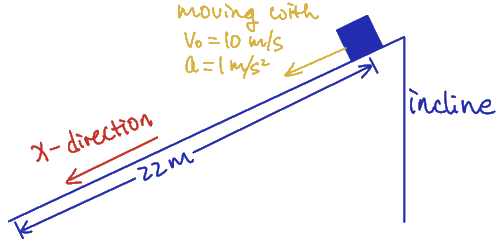
\includegraphics[width=0.45\textwidth]{incline}
%  \end{center}
%\end{wrapfigure}

%\noindent\textit{Example}:
%A box is sliding down from an incline (see figure). The acceleration of the box in the $x$-direction is $1$ m/s$^2$, and the initial velocity of the box in the $x$-direction is $10$ m/s. The incline is $22$ meters long. Find the time it takes to reach the bottom of the incline. \\
%
%Since we know the initial velocity $v_0 = 10$ m/s, the acceleration of the box $a = 1$ m/s$^2$, the initial position $x_0 = 0$ m, and the final position $x_{\text{f}} = 22$ m. We can apply the kinematic equation directly, 
%\begin{align*}
%22 = x_{\text{f}} = \frac{1}{2} a t^2 + v_0 t + x_0 = \frac{1}{2}t^2 + 10 t + 0\,.
%\end{align*}
%Then we use the quadratic formula (for the polynomial $0 = at^2 + bt + c$) to find $t$, 
%\begin{align*}
%t = \frac{-b \pm \sqrt{b^2 -4ac}}{2a} = \frac{-10 \pm \sqrt{100 + 44}}{1} = 2\,.
%\end{align*}
%So it takes $2$ \underline{seconds} for it to reach the bottom of the incline. You probably have noticed that $t = -22$ seconds is also a solution due to the $\pm$ signs in the quadratic formula. Why can we just ignore that $t=-22$ seconds solution?\\

\noindent\textit{Example}: 
Eric is working on an experiment in his Physics 5AL lab. He saw a ping-pong ball was initially moving to the right at a constant speed $1$ m/s for $2$ seconds. Then the ball hit the wall and moved back to the left at a constant speed $0.5$ m/s for another $5$ seconds. For now we ignore any friction.\\

In this case, we can set up the coordinate system with $x$-axis pointing to the right as usual. For the first two seconds, the ball moved to the right, so it had velocity $v_{\text{i}} = 1$ m/s. After the ball hit the wall, it moved to the left, so its velocity became $v_{\text{f}} = -0.5$ m/s (the negative sign indicates the direction to the left). The total \underline{distance} it has traveled (think about the mileage reading on a used car) is
\begin{align*}
|\Delta x| = |v_{\text{i}}| \cdot (2 \text{ s}) + |v_{\text{f}}|\cdot (5\text{ s}) = (1\ \text{m/s}) \cdot (2\text{ s}) +  (0.5\ \text{m/s}) \cdot (5\text{ s})  =4.5 \text{ m}\,.
\end{align*}
But the \underline{displacement} it has traveled is calculated differently, where we need to consider the ``net change" of its position in this case, 
\begin{align*}
\Delta x = v_{\text{i}} \cdot (2 \text{ s}) + v_{\text{f}}\cdot (5\text{ s}) = (1\ \text{m/s}) \cdot (2\text{ s}) +  (-0.5\ \text{m/s}) \cdot (5\text{ s}) = -0.5 \text{ m}\,. 
\end{align*}
This is because it ended at a position $0.5$ meters to the \underline{left} of where it started. Next we calculate the \underline{average speed} over the first $7$ seconds, 
\begin{align*}
\overline{s} = \frac{|\Delta x|}{7 \text{ s}} =\frac{4.5\ \text{m/s}}{7 \text{ s}}= 0.643 \ \text{m/s}\,.
\end{align*}
We don't care about the direction the ball was traveling when we calculate the average speed, but we do when we calculate its \underline{average velocity}:
\begin{align*}
\overline{v} = \frac{\Delta x}{7 \text{ s}}= \frac{-0.5\ \text{m/s}}{7 \text{ s}} = -0.071\,\text{m/s}\,.
\end{align*}
The acceleration of the ball in the first 2 seconds is $0$ m/s${}^2$, and also $0$ m/s${}^2$ after the ball has hit the wall. But at the instant the ball hit the wall, it was ``pushed" (hence accelerated)  to the left by the wall for a very short amount of time but with a very large magnitude, thus the velocity (and direction of motion) was changed. If we were to draw the velocity/position vs. time plot for this ball, we would have the followings.\\

\begin{center}
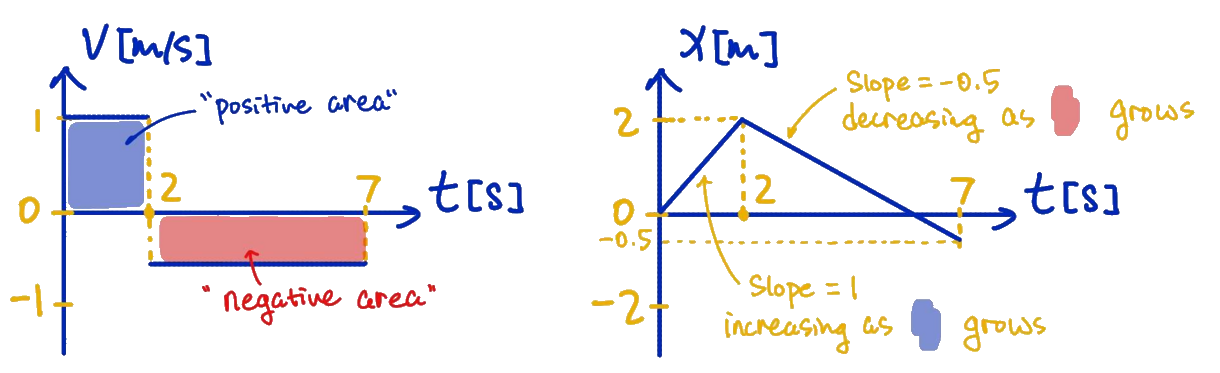
\includegraphics[width=1\textwidth]{eric}
\end{center}

Notice that the ``area" under the velocity curve (the shaded region bounded between the $x$-axis and the velocity curve, from $t=0$ to any other time) corresponds to the value of the position curve. The slope of the position curve corresponds to the value of the velocity curve. 


\newpage
\begin{center}
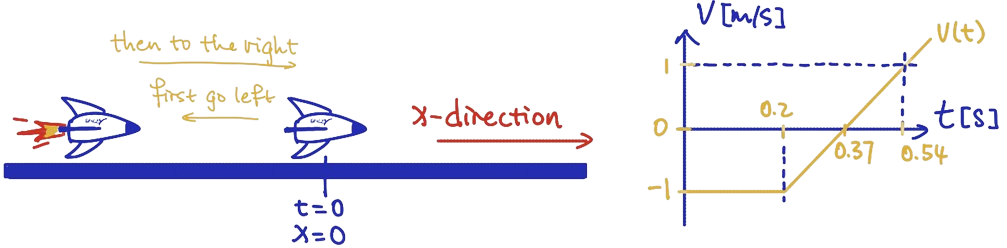
\includegraphics[scale=0.41]{rocket1}
\end{center}
\noindent \textbf{Problem 1}: A rocket is mounted on a track shown in the figure. The rocket initially has a speed moving to the left, then after a while the boost on the rocket is switched on, providing a constant acceleration to the right. Jinyan has obtained a velocity vs. time graph for the rocket as shown, and he asks you to draw the position vs. time, and acceleration vs. time graph for the rocket (You can assume that the position of the rocket at $t = 0$ s is $x =0$ m). Remember to label the axes. \\

\noindent (Hint: This problem is easy if you know calculus, but for Physics 5A, we guarantee that you can solve all problems without calculus. Think about "area under the curve" for finding the position plot, and "slope of the curve" for finding the acceleration plot.)
\newline\newline\newline
\newline\newline\newline
\newline\newline\newline




\noindent \textbf{Problem 2:} Calculate the displacement, traveled distance, average speed, and average velocity of the rocket in the first $0.54$ seconds. 
\newline\newline\newline
\newline\newline\newline
\newline\newline\newline


\noindent \textbf{Problem 3:} During the first 0.54 seconds, find the time instances that the rocket has (a) its highest speed, (b) highest velocity, (c) greatest displacement, (d) longest distance traveled.




%\begin{center}
%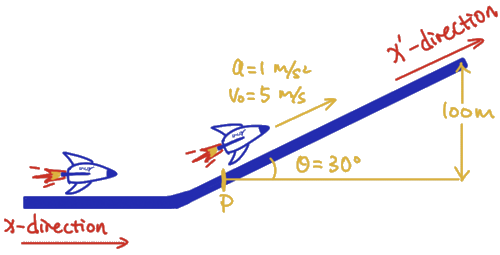
\includegraphics[scale=0.52]{rocket2}
%\end{center}
%\noindent \textbf{Problem 2}: After accelerating to the right for a few seconds, the rocket moves onto a ramp at an angle of $\theta = 30^\circ$. When it reaches point $P$ as shown, it has a velocity $v_0 = 5$ m/s in the $x'$-direction, but its acceleration in the $x'$-direction is down to $1$ m/s$^2$ due to gravity. How long does it take for the rocket to reach a height of $h = 100 $ m? \\
%
%\noindent(\textit{Hint: How far does the rocket need to travel in the $x'$-direction to reach $h=100$ m?})
%\newline\newline\newline
%\newline\newline\newline
%\newline\newline\newline
%\newline\newline\newline
%\newline\newline\newline
%\newline\newline\newline
%\noindent \textbf{Problem 3}: How far has the rocket traveled in the horizontal direction ($x$-direction) when it reaches $h = 100$ m. 

\newpage
\textbf{Problem 1 (solution)}: See the end of this file :)\\

\textbf{Problem 2 (solution)}: First we find the displacement, which is the ``net change" of the rocket's position in the first 0.54 seconds. This only involves two quantities, final position $x_\text{f}$ and initial position $x_{\text{i}}$ of the rocket. At $t=0.54$ seconds, we have $x_\text{f} = -0.2$ meters (obtained from the position graph). At $t = 0$ second, we have $x_\text{i} = 0$ meter. Then we can write
\begin{align*}
\text{Displacement} = x_\text{f} - x_\text{i} = (-0.2 - 0) \,\text{m} = -0.2 \,\text{m}
\end{align*} 
The traveled distance is like the mileage reading in your car, so the more time it spends running on the road, the longer the distance traveled. In this problem, the rocket traveled to the left for $0.2$ meters, continue to the left for $0.085$ meters, then to the right for $0.085$ meters, we add these three distances without negative sign, 
\begin{align*}
\text{Distance} = (0.2 + 0.085 + 0.085) \, \text{m}= 0.37 \, \text{m}
\end{align*}
Having displacement and distance calculated, average speed and average velocity can be calculated easily from their definitions. For average speed, 
\begin{align*}
\overline{s} = \frac{\text{Distance}}{\Delta t} = \frac{0.37\,\text{m}}{0.54\,\text{s}}= 0.685\,\text{m/s}\,.
\end{align*}
For average velocity
\begin{align*}
\overline{v} = \frac{\text{Displacement}}{\Delta t} = \frac{-0.2\,\text{m}}{0.54\,\text{s}} = 0.370\,\text{m/s}\,.
\end{align*}

\textbf{Problem 3 (solution)}: The speed of the rocket is the absolute value of its velocity, so we look at the velocity graph, we see that the rocket has speed $1$ m/s for the first $0.2$ seconds, and also has speed $1$ m/s at $t - 0.54$ s. At all other time, the rocket has speed less than $1$ m/s. \underline{(a) The rocket attains its highest speed at time between $0$ and $0.2$ seconds,} \underline{and also at $t=0.54$ seconds}. For highest velocity, we only look at the velocity plot and find its highest value, which is \underline{(b) $v=1$ m/s at time $t=0.54$ second}. Usually "highest velocity" is not a very useful, or informative, quantity because it does not account for the fact that the rocket can move to the left (negative velocity) at a very high speed, but it signifies highest speed towards the direction "you want" (the positive direction). Since the displacement of the rocket has a plus/minus sign, and based on the position graph, the displacement $\Delta x = x_\text{f} - x_{\text{i}} = x_{\text{f}}$ (because the rocket starts from $x_{\text{i}}$ at time $0$) is always negative, so the \underline{(c) largest number of displacement is $\Delta x = 0$ at time $t = 0$}. This is a tricky question, sometimes you might also be asked for the longest distance away from the origin, in which case is at time $0.38$, when the rocket is farthest to the left from where it started. The longest distance that the rocket has traveled (not the longest distance from the origin) has been calculated in problem 2, as the ``distance traveled" is like the mileage reading in your car, \underline{(d) the greatest number of that is at time $t=0.54$ s}. 


\includepdf[pages=-]{w1p1}

\end{document}


